% !TEX root = Projektdokumentation.tex
\section{Installationsanleitung}

\label{sec:tool_documentation}
\vspace*{36 pt}
\vspace{4cm}
\begin{center}\Huge\bfseries\itshape
BiLang-Zusatzsoftware: Installationsanleitung
\end{center}	

\vspace{11cm}
\begin{center}\large
	Version 1.0.0 vom 19.05.2021 \\
	Autor: \companyName
\end{center}

\newpage

\paragraph{1. Einleitung:}

Um eine Installation erfolgreich abzuschließen, befolgen Sie bitte sämtliche Schritte, die in dieser Anleitung anschaulich erklärt werden. Sie benötigen:

\begin{itemize}
	\item Zugangs- und Installationsrechte auf dem Windowssystem
	\item Zugangsdaten zu einem JTL-Wawi-Benutzer mit entsprechend hohen Rechten.
	\item Zugangsdaten zur JTL-Wawi-Datenbank
	\item Einen gültigen API-Schlüssel
	\item Die Software in der aktuellen Version zusammen mit den Ex- und Importvorlagen
\end{itemize}

\paragraph{2. Vorbereiten der Installation:}
Transferieren Sie die Software auf das Windowssystem auf dem auch die JTL-Wawi-Datenbank aktiv läuft.

\paragraph{3. Eigenes Feld anlegen:}
\begin{itemize}
	\item Erstellen Sie ein 'Eigenes Feld' das als Indentikator benutzt dafür verwerden werden kann, ob ein Artikel sich verändert hat oder nicht. 
	\item Wählen Sie dazu zuerst den Menüpunkt 'Admin -> Eigene Felder'.
	\item Legen Sie nun die 'RIS\_BiLang' Feldgruppe an, in der das Feld 'ArticleChanged' eingetragen wird. 
	\item Sie können außerdem unten links auswählen welche Warengruppen Sie übersetzen lassen möchten.
	\item Das Feld muss vom Datentyp 'Checkbox' sein, Anzeigeort und Beschreibung können frei gewählt werden.
	\item Bestätigen Sie Ihre Angaben, indem Sie die 'Speichern' Schaltfläche benutzen.
\end{itemize}

\begin{center}
	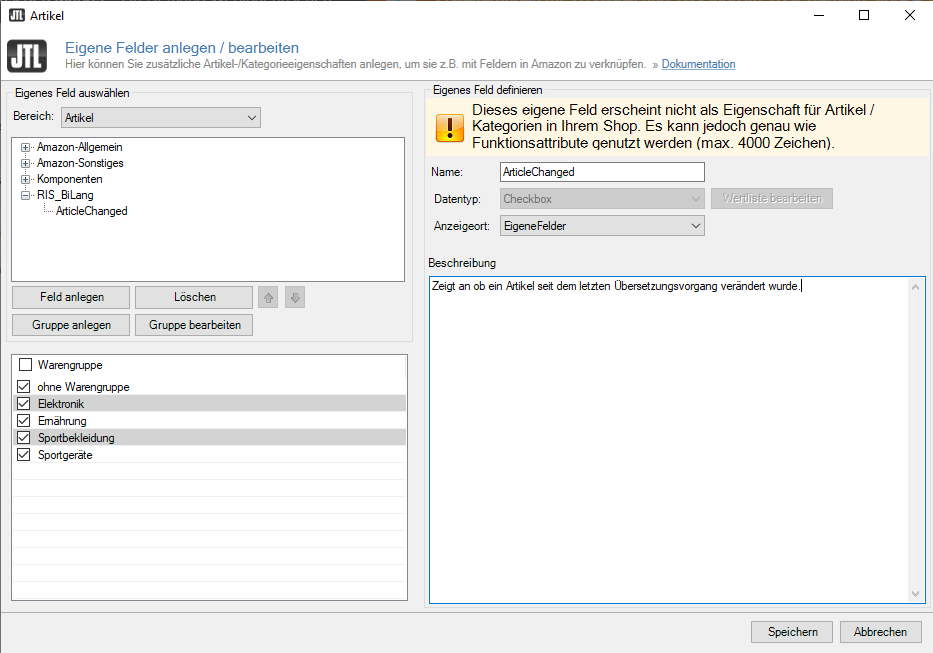
\includegraphics[width=9cm]{./img/eigenesFeld.png}
\end{center}

\paragraph{4. JTL-Wawi Workflow anlegen:}
Nun muss das soeben erstellte Feld benutzt werden, dazu wählen Sie wieder 'Admin' und nun 'JTL-Workflows':

\begin{itemize}
	\item Da das Feld immer dann auf Wahr gesetzt werden soll, wenn ein Artikel sich verändert hat, wird ein Workflow für das Ereignis 'Artikel - Geändert' erstellt.
	\item Die Bedingung kann verändert werden, es wird allerdings empfohlen keine Bedingung anzugeben.
	\item Erstellen Sie eine neue Aktion, indem Sie auf den entsprechenden Text klicken.
	\item Im Dropdown Menü wird die Option 'Werte setzen' ausgewählt und anschließend das 'ArticleChanged' als Variable gewählt.
	\item Bestätigen Sie Ihre Angaben, indem Sie die 'Speichern' Schaltfläche benutzen.
\end{itemize}
	
\begin{center}
	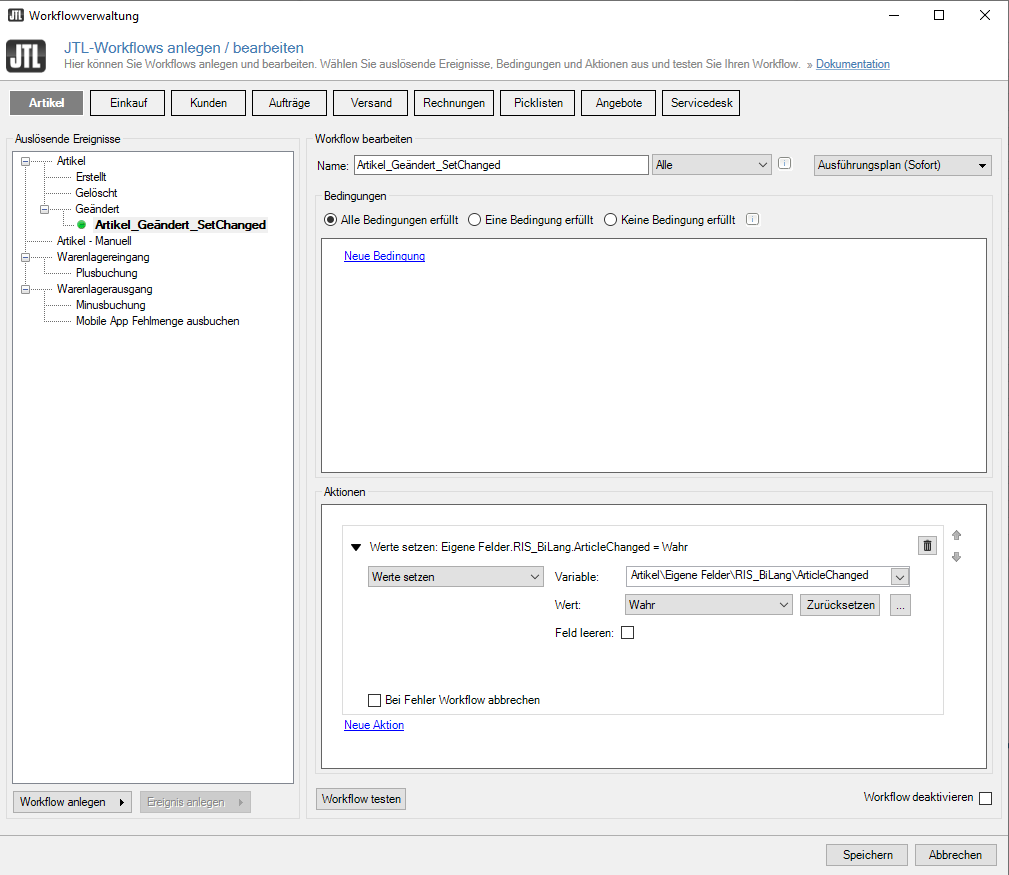
\includegraphics[width=9cm]{./img/workflows.png}
\end{center}

\paragraph{5. Konfigurationsdatei anpassen:}
Damit das Programm eine Verbindung zum JTL-Wawi Datenbankserver herstellen kann, muss die Konfigurationsdatei richtig beschrieben werden.
Im Bereich \texttt{appSettings} finden Sie verschiedene Punkte. 

\texttt{db\_server} : Die IP-Adresse des Datenbankservers mit der Instanz der JTL-Wawi-Datenbank als Anhang, getrennt durch einen ``\textbackslash''.

\texttt{db\_port} : Der Port unter dem die Datenbank angesprochen werden kann.

\texttt{db\_mandant} : Der Name des Mandanten für den die Übersetzung aktiviert werden soll.

\texttt{db\_user} : Der Benutzername zu einem Datenbankbenutzer (Standardwert 'sa').

\texttt{db\_pass} : Das Passwort zum Datenbankbenutzername in db\_user (Standardwert 'sa04jT14').

\texttt{jtlAmeisePath} : Der absolute Pfad zur 'JTL-wawi-ameise.exe', welche im Installationsverzeichnis liegt (Standardwert 'C:\textbackslash Programme\textbackslash JTL-Software\textbackslash JTL-wawi-ameise.exe').

Außerdem können die \texttt{appLanguages} nach Belieben ein- oder auskommentiert werden, um diese auch tatsächlich zu nutzen.

\paragraph{6. Windows-Aufgabenplanung konfigurieren:}%
Um das Programm automatisiert starten zu lassen, verwenden Sie die Windows-Aufgabenplanung. 
Diese ermöglicht Programmstarts mit festen Intervallen.

\begin{center}
	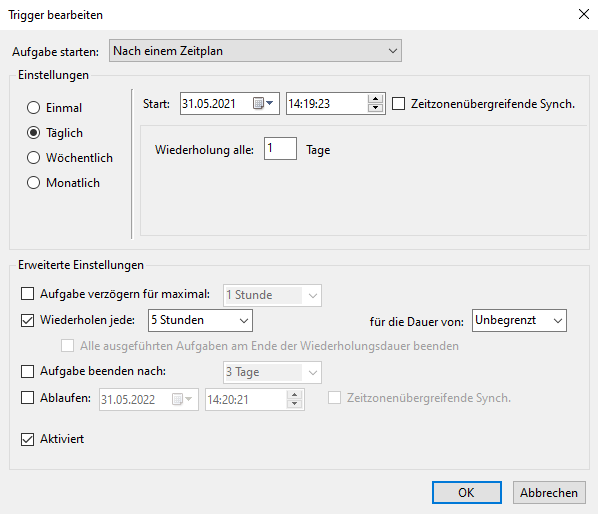
\includegraphics[width=9cm]{./img/Aufgabenplanung3.png}
\end{center}

\begin{itemize}
	\item Dazu müssen Sie eine 'Aufgabe erstellen...'
	\item Name und Beschreibung ist frei wählbar
	\item Wechseln Sie in den Reiter 'Trigger' und legen einen neuen Trigger an
\end{itemize}

\begin{center}
	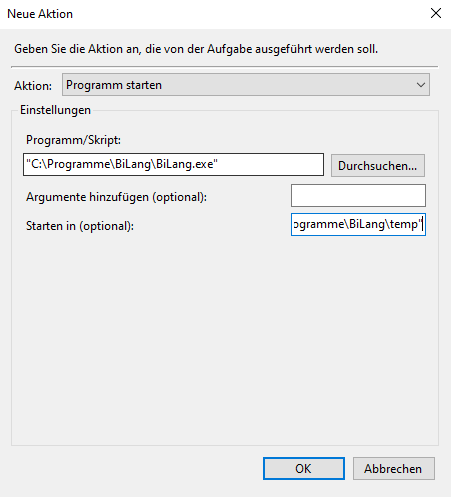
\includegraphics[width=8cm]{./img/Aufgabenplanung2.png}
\end{center}

\begin{itemize}
	\item Hier wird angegeben, wie oft das Programm eine Übersetzung anstoßen soll. Empfohlen wird eine Tägliche Ausführung, sowie manuelle Starts bei großen Veränderungen in den Stammdaten der JTL-Wawi.
	\item Nach eine Bestätigung mit OK, können Sie auf den Reiter 'Aktionen' wechseln. 
	\item Hier erstellen Sie eine neue Aktion vom Typ 'Programm starten' und wählen die BiLang.exe aus Ihrem Verzeichnis aus.
	\item Empfohlen wird in dem Feld 'Starten in' den absoluten Pfad des Verzeichnisses 'BiLang/temp' auszuwählen.
\end{itemize}